% !TeX root = ../mat_mod2.tex

\section{
  Маршрут резки и оптимизационные задачи
  маршрутизации инструмента машин листовой
  резки с~ЧПУ
}
\label{sect:1.2}
\setcounter{equation}{0}

Для формального определения маршрута резки
введем следующие обозначения.
Пусть
$A_1, A_2, \,\dots, A_n$
– двумерные геометрические объекты (точечные замкнутые множества),
представляющие собой односвязные или
многосвязные области эвклидовой плоскости
$\mathbb R \times \mathbb R$,
ограниченные одной или несколькими замкнутыми кривыми
(граничными контурами)
$C_1, C_2, \,\dots, C_N$
$(A_i, C_J \subset \mathbb R \times \mathbb R;
i \in \overline{1,n};
j \in \overline{1, N};
N \geqslant n)$.
Объекты
$A_1, A_2, \,\dots, A_n$
являются геометрическими моделями плоских заготовок/деталей
({\it в дальнейшем в книге термин <<деталь>>,
которая вырезается из листового материала,
будет использоваться как синоним термина <<заготовка>>}).

Пусть также определена область размещения объектов
$B \subset \mathbb R \times \mathbb R$,
которая является геометрической моделью листового материала,
из которого вырезаются детали.
В общем случае область размещения
может содержать несколько кусков материала
(не обязательно прямоугольной формы),
но для решения оптимизационных задач
маршрутизации инструмента целесообразно рассматривать
в качестве области размещения одно замкнутое точечное множество,
ограниченное (как и деталь)
одним внешним контуром.
При этом допустимо наличие отверстий в материале
(внутренних контуров).
Будем полагать, что зафиксирован некоторый вариант размещения
объектов в области размещения,
при этом выполнены условия взаимного непересечения объектов.
Полагаем также, что выполнены другие дополнительные условия,
обусловленные технологическими требованиями резки деталей
на конкретном технологическом оборудовании с ЧПУ,
в частности, условие соблюдения необходимой ширины реза.
Другими словами, фиксированный вариант размещения объектов
является допустимым вариантом раскроя листового материала
для заданного набора $n$ деталей.

Пример размещения в прямоугольной области 24 объектов
($n=24$),
описываемых 30 замкнутыми контурами
($N=30$)
с заданным минимальным расстоянием между объектами,
приведен на рис.~\ref{nesting}.

\begin{figure}[h]
  \begin{center}
  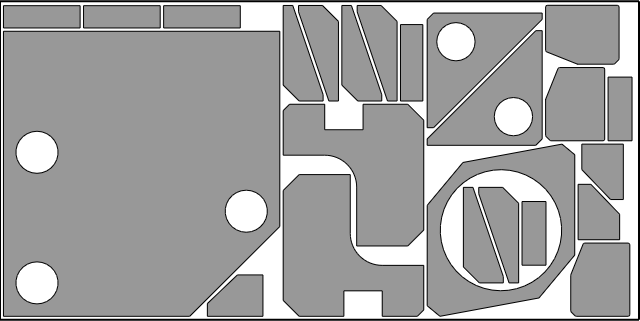
\includegraphics[width=0.9\textwidth]{nesting.png}
  \caption{Пример раскроя листа $2000 \times 1000$ мм с заданным минимальным расстоянием между деталями 10 мм}
  \label{nesting}
  \end{center}
\end{figure}

Раскройная карта
на рис.~\ref{nesting}
получена с помощью подсистемы автоматического раскроя
\textit{CAD/CAM}
системы <<Сириус>>.

Предположим, что для вырезки деталей было использовано
$K$
сегментов резки
$S_k=M_kM^*_k; k \in \overline{1,K}$.
Тогда маршрут резки деталей можно определить
в терминах сегментов резки как кортеж
\begin{equation}
  ROUTE = \left<
    M_0, M_1, S_1, M_1^*, M_2, S_2, M_2^*, \,\dots, M_K, S_K, M_K^*,
    i_1, i_2, \,\dots, i_K
  \right>
  ,
  \label{tuple}
\end{equation}
где
$M_0$
-- начальная точка положения инструмента,
$i_1, i_2, \,\dots, i_K$
– последовательность, в которой вырезаются используемые сегменты резки
$S_1, S_2, \,\dots, S_K$.
Линейное перемещение инструмента на холостом ходу
между точкой выключения инструмента и следующей точкой врезки
однозначно определяется этой последовательностью.
Если применить комбинаторную терминологию,
то последовательность однозначно задается перестановкой порядка
$K$,
т. е. упорядоченным набором натуральных чисел от $1$ до $K$
(биекцией на множестве $\overline{1,K}$),
которая числу
$k \in \overline{1,K}$
ставит в соответствие элемент
$i_k$ из набора.
Отметим, что термин <<маршрут резки>> является
общепринятым технологическим понятием.
В главах 3 -- 5 при описании математических моделей оптимизации
маршрута резки мы будем использовать термин <<маршрут>>
применительно к перестановке
$i_1, i_2, \,\dots, i_K$,
что, в свою очередь, соответствует устоявшейся
терминологии в задаче о последовательном обходе мегаполисов.

На рис.~\ref{cutting}
показана схема одного из возможных маршрутов резки для примера,
приведенного на рис.~\ref{nesting}.

\begin{figure}[h]
  \begin{center}
  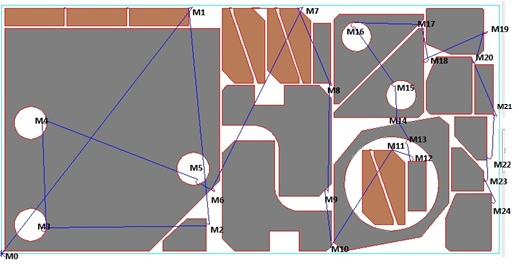
\includegraphics[width=0.9\textwidth]{cutting.png}
  \caption{Пример маршрута резки, содержащего 24 сегмента резки}
  \label{cutting}
  \end{center}
\end{figure}

Маршрут резки содержит 24 сегмента.
Для резки внешних контуров трех групп деталей
с точками врезки $M_1$
(три детали в группе),
$M_7$
(четыре детали в группе) и
$M_{11}$
была использована мультиконтурная резка
(указанные группы деталей выделены коричневым цветом).
Все остальные контуры вырезаны с применением стандартной техники резки.
Последовательность резки сегментов соответствует
номерам точек врезки $M_J$ ($J=1,2,\,\dots, 24$).
После вырезки последнего сегмента
возврат инструмента в начальную точку $M_0$
не программировался.

На приведенном рис.~\ref{cutting}
визуализация траектории инструмента
осуществляется точно по граничным контурам деталей,
а не по их эквидистантным контурам, хотя,
как отмечено выше,
траектория реза должна отстоять от
граничного контура на половину ширины реза.
Это связано с тем, что в большинстве
\textit{CAM}-систем
(\textit{Computer Aided Manufacturing})
программирование движения инструмента первоначально
осуществляется по граничным контурам деталей,
а вычисление реальной траектории производится
либо непосредственно самой системой ЧПУ,
либо специальной программой-постпроцессором,
предназначенной для конвертирования информации о
маршруте резки из внутреннего формата системы в
формат команд конкретного технологического оборудования с ЧПУ.
В этом случае величину припуска на рез
устанавливает оператор на станке перед запуском
управляющей программы резки.

В дальнейшем без ограничения общности мы будем полагать,
что траектория инструмента в маршруте резки $ROUTE$
программируется по граничным контурам,
и сегменты резки
$S_k=M_kM^*_k; k \in \overline{1,K}$
содержат все граничные контуры деталей
$C_1, C_2, \,\dots, C_N$,
т. е.
$$
\bigcup_{j=1}^N C_j \subset \bigcup_{k=1}^K S_k
$$

Соответственно, все точки входа в эквидистантный контур
(и выхода из эквидистантного контура)
также лежат на граничных контурах,
см. рис.~\ref{standard-cutting}.

На рис.~\ref{control-program}
показан фрагмент управляющей программы
($G$-кода) для машины листовой газовой резки
типа <<Комета>> с системой ЧПУ 2Р32М.

\begin{figure}
\begin{multicols}{3}

  \%УП\_2Р32М\_01
  N1G91 \\
  N2G00X7662Y9909F6000 \\
  N3M70T1 \\
  N4M71T1 \\
  N5G01X-141Y-48F460 \\
  N6X-2400  \\
  N7X-40  \\
  N8X-67  \\
  N9X-2400  \\
  N10X-40 \\
  N11X-67 \\
  N12X-2400 \\
  N13Y-700  \\
  N14X2400  \\
  N15Y700 \\
  N16Y40  \\
  N17X107Y-40 \\
  N18Y-700  \\
  N19X2400  \\
  N20Y700 \\
  N21Y40  \\
  N22X107Y-40 \\
  N23Y-700  \\
  N24X2400  \\
  N25Y700 \\
  N26Y40  \\
  N27M74T1  \\
  N28G00X817Y-8745F6000 \\
  N29M71T1  \\
  N30G03X-108Y0I-54J0F460 \\
  N31G01Y-1048  \\
  N32X-1740 \\
  N33Y400 \\
  N34X940Y900 \\
  N35X800 \\
  N36Y-252  \\
  N37X20Y-30  \\
  … \\
  N314M71T1 \\
  N315G02X-130Y0I-65J0F460  \\
  N316G01Y267 \\
  N317G03X-50Y50I-50J0  \\
  N318G01X-1366 \\
  N319G03X-46Y-31I0J-50 \\
  N320G01X-384Y-960 \\
  N321G03X-4Y-19I46J-19 \\
  N322G01Y-1120 \\
  N323G03X14Y-35I50J0 \\
  N324G01X122Y-121  \\
  N325G03X37Y-14I35J35  \\
  N326G01X1627Y-1 \\
  N327G03X50Y50I0J50  \\
  N328G01Y1933  \\
  N329X20Y30  \\
  N330M74T1 \\
  N331M75T1 \\
  N332M02 \\
  M30
\end{multicols}
\caption{Фрагмент УП для машины листовой резки <<Комета>> с ЧПУ 2Р32М }
\label{control-program}
\end{figure}

Программа сгенерирована на основе маршрута резки
(спроектированного в интерактивном режиме в
\textit{CAD/CAM} системе <<Сириус>>
и показанного на рис.~\ref{cutting})
соответствующим постпроцессором со
следующими числовыми параметрами резки:
\begin{itemize}
  \item	число строк в УП – 333;
  \item	количество точек врезки (пробивки листа) – 24;
  \item	путь инструмента на рабочей скорости – 27,36 м;
  \item	путь инструмента на быстром (холостом) ходу – 8,39 м;
  \item	время движения на рабочей скорости – 62,04 мин;
  \item	время движения на быстром (холостом) ходу – 1,64 мин;
  \item	общее время резки: 63,68 мин.
\end{itemize}

В зависимости от выбранного маршрута резки
числовые параметры резки могут существенно различаться.
Таким образом, при разработке управляющих программ
для машин фигурной листовой резки с ЧПУ возникают
различные задачи оптимизации маршрута инструмента.
В качестве критерия оптимизации (целевой функции)
в этих задачах чаще всего рассматривается общее время резки.
При термической и гидроабразивной резке для сформированного
маршрута резки общее время резки
$T_{cut}$
рассчитывается по следующей формуле:
\begin{equation}
  T_{cut} = \frac{L_{on}}{V_{on}} + \frac{L_{off}}{V_{off}} +N_{pt} \cdot t_{pt}
  ,
  \label{cutting-time}
\end{equation}
где
$L_{on}$ -- длина реза с включенным режущим инструментом;
$V_{on}$ -- скорость рабочего хода режущего инструмента;
$L_{off}$ -- длина переходов с выключенным режущим инструментом (холостой ход);
$V_{off}$ -- скорость холостого хода;
$N_{pt}$ -- количество точек врезки;
$t_{pt}$ -- время, затрачиваемое на одну точку врезки.
При этом подразумевается,
что получаемое в результате врезки отверстие
расположено внутри материала листа.
Однако при резке заготовок, как отмечалось,
могут быть использованы и другие типы врезки,
что приводит к изменению времени врезки
$t_{pt}$
в этих случаях.
Если при резке деталей было использовано несколько типов врезки,
то формула~(\ref{cutting-time}) запишется в более общем виде:
\begin{equation}
  T_{cut} = \frac{L_{on}}{V_{on}} + \frac{L_{off}}{V_{off}} +
  \sum_{j=1}^p N_{pt}^j \cdot t_{pt}^j
  ,
  \label{cutting-time-multi}
\end{equation}
где
$p$ -- число использованных типов врезки,
$N_{pt}^j$ -- количество точек врезки типа $j$;
$t_{pt}^j$ -- время, затрачиваемое на одну точку врезки типа $j$.

И в (\ref{cutting-time})
и в (\ref{cutting-time-multi})
значение скорости холостого хода инструмента
$V_{off}$ -- константа,
определяемая техническими характеристиками
используемого технологического оборудования.
Значение скорости рабочего хода инструмента
$V_{on}$
программируется при разработке управляющей программы
в соответствии с используемой технологией резки
и параметрами листового материала
(марка материала и толщина).
Предполагается, что заданная величина
$V_{on}$  в (\ref{cutting-time}) и в (\ref{cutting-time-multi})
также является константой,
однако на практике фактическая скорость резки
может меняться в зависимости от различных технологических факторов,
а также характеристик спроектированной управляющей программы.
Это диктует необходимость проведения исследований для
определения поправочного коэффициента для величины
$V_{on}$.
В \ref{sect:1.4}
приведены результаты такого рода исследований
применительно к машине лазерной резки с ЧПУ
\textit{ByStar 3015}
для листового материала
\textit{АМг3М} толщиной от 1,5 до 5 мм.

Важнейшей экономической характеристикой качества
разработанной управляющей программы является стоимость
(себестоимость) резки деталей на машине с ЧПУ.
Это сложный интегрированный показатель,
который включает в себя произведенные во время
резки затраты на электроэнергию и расходные материалы,
на обслуживание машины с ЧПУ,
а также другие эксплуатационные затраты.
Отметим, что стоимость резки не всегда
пропорциональна времени резки,
поскольку зависит еще и от различных режимов резки.
По аналогии с формулой времени резки (\ref{cutting-time})
показатель стоимости резки можно определить по следующей формуле:
\begin{equation}
  F_{cost}=
  L_{on} \cdot C_{on} +
  L_{off} \cdot C_{off} +
  N_{pt} \cdot C_{pt}
  ,
  \label{cutting-cost}
\end{equation}
где
$C_{on}$ -- стоимость единицы пути с включенным режущим инструментом;
$C_{off}$ -- стоимость единицы пути с выключенным режущим инструментом;
$C_{pt}$ -- стоимость одной точки врезки,
а $L_{on}, L_{off}, N_{pt}$
имеют тот же смысл, что и в формуле~(\ref{cutting-time}).
При этом $C_{on}, C_{off}, C_{pt}$ --
величины, зависящие от типа машины с ЧПУ,
технологии резки, используемой скорости рабочего хода инструмента,
толщины и марки материала.
Функциональная зависимость
$C_{on}, C_{off}, C_{pt}$
от перечисленных параметров
может задаваться либо табличными функциями,
либо аналитически.
При этом абсолютные значения этих величин
на российских предприятиях, использующих машины с ЧПУ,
определяются экономическими службами с учетом многих факторов
и могут существенно различаться на разных предприятиях.
Зачастую стоимость резки вообще не учитывается
в раскройно-заготовительном производстве,
либо рассчитывается на основании специальных нормативов,
не зависящих от величин
$L_{on}, L_{off}, N_{pt}$.

Очевидно, что необходимость расчета стоимости резки
для каждой управляющей программы резки возникает на предприятиях,
оказывающих услуги сторонним организациям по резке материала.
Однако и на многих таких предприятиях для определения
стоимости резки учитывается только длина рабочего хода инструмента
$L_{on}$,
которая принимается равной суммарному периметру граничных контуров вырезаемых деталей
$C_1, C_2, \,\dots, C_N$,
что, естественно, приводит к неадекватной оценке эффективности процесса резки.
В дальнейшем при оптимизации стоимостных параметров резки
мы будем применять теоретически обоснованный способ определения
показателя стоимости резки, задаваемый формулой (\ref{cutting-cost}).

На рис.~\ref{cost} представлен расчет стоимости резки
$F_{cost}$
для рассматриваемого примера при резке деталей на машине газовой резки.
Значения величин
$C_{on}, C_{off}, C_{pt}$
взяты из таблицы, используемой для расчета себестоимости фигурной
листовой резки на одном из предприятий Свердловской области.

\begin{figure}[h]
  \begin{center}
  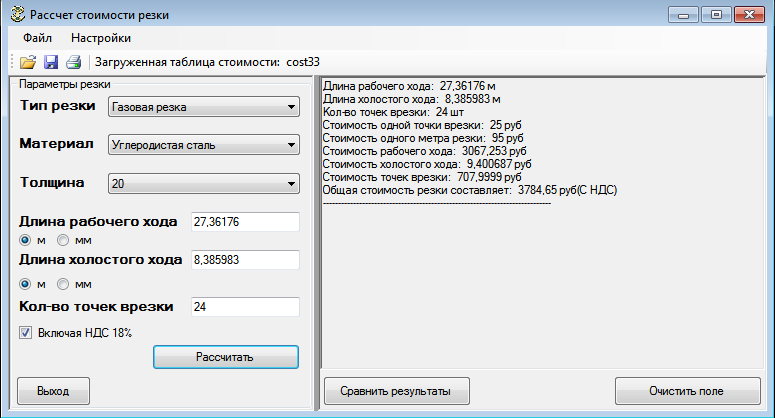
\includegraphics[width=0.9\textwidth]{cost.png}
  \caption{
    Пример расчета стоимости резки $F_{cost}$
    при резке деталей из~углеродистой стали
    толщины 20~мм на~машине газовой резки}
  \label{cost}
  \end{center}
\end{figure}

Следует отметить,
что задача правильного определения величин
$C_{on}$, $C_{off}$, $C_{pt}$
для конкретного технологического оборудования
и конкретного материала сама по себе является малоисследованной проблемой.
В \ref{sect:1.4}
приведены результаты исследования,
позволяющего точно вычислять себестоимость
лазерной резки применительно для машины с ЧПУ
\textit{ByStar3015}
при резке углеродистой и нержавеющей
стали различных толщин
(на примере Ст10кп и 12Х18Н10Т),
а также при резке алюминия и его сплавов
(на примере \textit{Амг3М}).

В случае использования нескольких типов врезки формула~(\ref{cutting-cost}) примет вид:
\begin{equation}
  F_{cost}=
  L_{on} \cdot C_{on} +
  L_{off} \cdot C_{off} +
  \sum_{j=1}^p N_{pt}^j \cdot C_{pt}^j
  ,
  \label{cutting-cost-multi}
\end{equation}
где $C_{pt}^j$ -- стоимость одной точки врезки типа $j$.

Как легко заметить,
значения целевых функций (\ref{cutting-time}) -- (\ref{cutting-cost-multi})
однозначно определяются маршрутом резки,
задаваемым кортежем (\ref{tuple}),
поскольку геометрия сегментов резки
$S_1, S_2, \,\dots, S_K$
позволяет вычислить длину рабочего хода инструмента  $L_{on}$,
а координаты точек
$M_0$, $M_1$, $M_1^*$, $M_2$, $M_2^*$, \,\dots, $M_K$, $M_K^*$
и перестановка
$i_1$, $i_2$, \,\dots, $i_K$
(последовательность, в которой вырезаются используемые сегменты резки)
задают набор холостых перемещений инструмента,
который определяет суммарную длину холостого хода
$L_{off}$.

Таким образом, сформулированные задачи оптимизации
маршрута инструмента для машин фигурной листовой резки с ЧПУ
можно представить в самом общем виде
как задачу минимизации некоторой числовой функции $F$,
заданной на множестве $G$ допустимых кортежей $ROUTE$,
т. е.
\begin{equation}
  F(ROUTE) \to \min_{ROUTE \in G}
  .
  \label{problem-statement}
\end{equation}

Поскольку элементы кортежа содержат
(помимо последовательности резки
$i_1, i_2, \,\dots, i_K$,
выбираемой из дискретного множества перестановок)
точки врезки и точки выключения инструмента
$M_kM_k^*, k \in \overline{1,K}$,
которые, в свою очередь,
могут быть выбраны из континуальных подмножеств евклидовой плоскости
$\mathbb R \times \mathbb R$,
даже в случае наложения существенных ограничений
на возможность выбора допустимых сегментов
$S_k$
оптимизационная задача (\ref{problem-statement})
может быть отнесена к классу очень сложных задач
непрерывно-дискретной оптимизации.
Некоторые вопросы формирования допустимых сегментов резки мы рассмотрим в части 2
настоящей монографии при математической формализации задачи (\ref{problem-statement})
и ее сведении к задаче о последовательном обходе мегаполисов.
В следующем параграфе мы сформулируем основные ограничения
на допустимые значения элементов последовательности резки
$i_1, i_2, \dots i_K$
и на значения
$M_kM_k^*, k \in \overline{1,K}$,
вызванные особенностями технологии листовой резки на машинах с ЧПУ.
